%\documentclass[a4paper, twoside, draft]{report}
\documentclass[a4paper]{report}
% ### PACKAGES ###
% ENCODING
\usepackage[utf8]{inputenc}
% FANCY HEADER CONFIGURATION
\usepackage{fancyhdr}
\pagestyle{fancy}
\renewcommand{\chaptermark}[1]{%
	\markboth{\MakeUppercase{#1}}{}}
	\renewcommand{\sectionmark}[1]{%
	\markright{\thesection\ #1}}
\fancyhf{} % delete current header and footer
\fancyhead[LE,RO]{\bfseries\thepage}
\fancyhead[LO]{\bfseries\rightmark}
\fancyhead[RE]{\bfseries\leftmark}
\renewcommand{\headrulewidth}{0.5pt}
\renewcommand{\footrulewidth}{0pt}
\addtolength{\headheight}{0.5pt} % space for the rule
\fancypagestyle{plain}{%
	\fancyhead{} % get rid of headers on plain pages
	\renewcommand{\headrulewidth}{0pt}} % and the line
% FANCY REF
\usepackage[english]{fancyref}
\newcommand*{\fancyreflstlabelprefix}{alg}
\fancyrefaddcaptions{english}{%
  \providecommand*{\freflstname}{algorithm}%
  \providecommand*{\Freflstname}{Algorithm}%
}
\frefformat{plain}{\fancyreflstlabelprefix}{\freflstname\fancyrefdefaultspacing#1}
\Frefformat{plain}{\fancyreflstlabelprefix}{\Freflstname\fancyrefdefaultspacing#1}
\frefformat{vario}{\fancyreflstlabelprefix}{\freflstname\fancyrefdefaultspacing#1#3}
\Frefformat{vario}{\fancyreflstlabelprefix}{\Freflstname\fancyrefdefaultspacing#1#3}
% KTH TITLE PAGE
\usepackage{KTHEEtitlepage}
% BIBLIOGRAPHY IN TOC
\usepackage{tocbibind}
% APPENDIX
\usepackage[toc,page]{appendix}
% BIBTEX
\usepackage{cite}
% PARSKIP
%\usepackage[parfill]{parskip}
% MATH TOOLS
\usepackage{mathtools}
\usepackage{amssymb} %for /neqsubset
\usepackage{commath} %for abs values
\usepackage{amsthm}  %for lemma and proof
\newtheorem{theorem}{Theorem}[section]
\newtheorem{lemma}[theorem]{Lemma}
% MATH SYMBOLS
\renewcommand{\S}{\mathbb{S}}
\newcommand{\R}{\mathbb{R}}
\newcommand{\calW}{\mathcal{W}}
\newcommand{\calA}{\mathcal{A}}
\newcommand{\calC}{\mathcal{C}}
\newcommand{\calO}{\mathcal{O}}
\newcommand{\calP}{\mathcal{P}}
\newcommand{\calL}{\mathcal{L}}
\newcommand{\calF}{\mathcal{F}}
\newcommand{\bldx}{\mathbf{x}}
\newcommand{\calx}{\mathcal{x}}
\newcommand{\bldo}{\mathbf{o}}
\newcommand{\blde}{\mathbf{e}}
% ALGORITHM
\usepackage{algorithm}
% PSEUDO CODE
\usepackage{algpseudocode}
% FIGURES
\usepackage{xcolor,graphicx}
\usepackage{epstopdf}
% PLOTS
\usepackage{pgfplots}
\graphicspath{ {figures/} }
% CUSTOM --> Command to include EPS images with latex text replacement
\newcommand{\includegraphicsTex}[2][\textwidth]{\def\svgwidth{#1}\input{figures/#2}}
% HYPERREF
\usepackage[pagebackref]{hyperref}
\definecolor{urlcolor}{HTML}{1954a6}
\definecolor{linkcolor}{HTML}{24a0d8}
\definecolor{citecolor}{HTML}{b0c92c}
\hypersetup{
% PDF SPECIFIC
    pdftitle={Path Planning for the KTH Research Concept Vehicle},
    pdfauthor={Karl Kurzer},
    pdfsubject={Path Planning},
    pdfkeywords={path planning, hybrid a star, hybrid a*},
    pdfnewwindow=true,
% COLORS
    colorlinks=true,
    linkcolor=linkcolor,
    citecolor=citecolor,
    urlcolor=urlcolor
}

\begin{document}
% TITLE PAGE
\ititle{Path Planning for the KTH \mbox{Research Concept Vehicle}}
\isubtitle{A Hybrid A* Approach}
\iauthor{Karl Kurzer}
\idate{July 2016}
\iaddress{Integrated Transport Research Lab\\School of Science\\KTH Royal Institute of Technology}
\makeititle

% ROMAN
\pagenumbering{roman}
% TABLE OF CONTENTS
\setcounter{tocdepth}{1}
\tableofcontents
% LIST OF FIGURES
\listoffigures
% LIST OF ALGORITHMS
\listofalgorithms

% ABSTRACT
\begin{abstract}
On the way to fully autonomously driving vehicles a multitude of challenges have to be overcome. One common problem is the navigation of the vehicle from a start pose to a goal pose in an environment that does not provide any specific structure (no defined lanes). Typical examples of such environments are parking lots or construction sights; in these scenarios the vehicle needs to navigate safely around obstacles ideally using the optimal (with regard to a specified parameter) path between the start and the goal pose.

The work conducted throughout this master's thesis focuses on the development of a suitable path planning algorithm for the Research Concept Vehicle (RCV) of the Integrated Transport Research Lab (ITRL) at KTH Royal Institute of Technology, in Stockholm, Sweden.

The development of the path planner requires more than just the pure algorithm, as the code needs to be tested and respective results evaluated. In addition, the resulting algorithm needs to be wrapped in a way that it can easily be deployed and interfaced with different other systems on the research vehicle. Thus the thesis also tries to gives insights into ways of achieving real-time capabilities necessary for experimental testing as well as on how to setup an visualization environment for simulation and debugging.
\end{abstract}

\pagenumbering{arabic}
\part{Introduction and Theoretical Framework}
% INTRODUCTION
\chapter{Introduction}
On the way to fully autonomously driving vehicles a multitude of challenges have to be overcome. A crucial part for autonomously driving vehicles is a planning system that typically encompasses different abstraction layers, such as mission, behavioral, and motion planning. While the mission planner provides a suitable route in a road network to arrive at the goal, the behavioral planner determines appropriate actions in traffic, such as changing lanes as well as stopping at intersections; the motion planner on the other hand operates on a lower level, avoiding obstacles, while progressing towards local goals \cite{Urmson.2008}.

An even more specialized problem is the navigation of the vehicle from a start pose to a goal pose in an environment that does not provide any specific structure; unstructured driving as opposed to structured driving (road following). Typical examples of such environments are parking lots or construction site. In these scenarios the vehicle needs to navigate safely around obstacles without any kind of path reference, such as lane markings, ideally using the optimal\footnote{with regard to a specified parameter, such as time, length, velocity, lateral acceleration, distance to obstacles, etc.}path between the start and the goal pose.

\section{Relevance of the Topic}
Autonomous driving vehicles might be one of the most publicly discussed and researched engineering topics at the moment of this writing. While the traditional car makers seem to pick up speed only very slowly, new entrants such as Alphabet (formerly Google) Comma.ai, drive.ai, Uber in the USA as well as OXBOTICA in the UK, and ZMP, Robot Taxi and nuTonomy in Asia are accelerating the advancement in self driving car technology at a rapid pace, releasing autonomous vehicles before the decade's end. A simple query with the search term \emph{autonomous driving} on Google Trends will underline this, revealing a huge increase in search volume over the past six years depicted in \Fref{fig:googleTrends}.

In a study titled ''Revolution in the Driver's Seat: The Road to Autonomous Vehicles'' the Boston Consulting Group defines Tesla's Autopilot released in October 2015 the first stage of several from partial to fully autonomous driving. Furthermore their estimates are, that fully autonomous driving vehicles will arrive by 2025. The most cited reasons by consumers in the USA to purchase an autonomous driving vehicle were an increase in safety, lower insurance premiums as well as the ability to be productive and multitask while the vehicle is driving. \cite{Mosquet.2015} 

For the society at large the most important benefit will be the reduction of accidents, as 90 percent of the time human error accounts for these. Other benefits of self-driving cars are the reduction of space consumption necessary for parking (self-driving cars don't need space to open the doors, which accounts to roughly 15\%) as reported by McKinsey \& Company. \cite{Bertoncello.2015}

\begin{figure}[h]
%\includegraphicsTex{MF.eps_tex}
\begin{tikzpicture}
	\begin{axis}[
		height=5cm,
		width=\textwidth,
		xlabel=Year, ylabel=Relative Frequency,
		xtick={40,197, 354, 510},
		xticklabels={Apr 2007, Apr 2010, Apr 2013, Apr 2016},
		]
		\addplot [black, mark=none]
		table [col sep=comma, x=week, y=freq] {figures/google_trends.dat};
%		\addplot [black, mark=-]
%		table[col sep=comma, x=week, y={create col/linear regression={y=freq}}] {figures/google_trends.dat};
	\end{axis}
\end{tikzpicture}
\caption{Google Trends for the query ``autonomous driving''}
\label{fig:googleTrends}
\end{figure}

\section{Context of the Thesis}
The Integrated Transport Research Lab (ITRL) at KTH is responding to the need for long-term multidisciplinary research cooperation to tackle the global environmental transport challenges by means of radically new and holistic technical solutions. Our approach is that seamless transport services, infrastructure, novel vehicle concepts, business models and policies, all need to be tuned and optimized in chorus.

A key role for the research of new technical solutions at the ITRL is the Research Concept Vehicle (RCV), that serves as a test bed for a variety of research topics, that cover areas of the vehicle such as, design, control, perception, planning as well as systems integration.

As autonomous driving will be a part of the solution for global environmental transport challenges the aim with this and other theses is to equip the RCV step by step with the capabilities to become self-driving. Hence this thesis will be a part of a much larger project.

\section{Problem Description} \label{sec:problemDescription}
The problem that this thesis aims to solve can be summarized as follows.

\emph{Find a solution in real-time that transitions a nonholonomic vehicle collision free from a given start pose to a desired goal pose within an unstructured environment based on the input of a two dimensional obstacle map, or report the existence of such a solution.}

\Fref{fig:problemDepiction} depicts the problem. The path transitions the vehicle from the start state $x_s$ safely to the goal state $x_g$, while adhering to the minimal turning radius $r$ of the vehicle and avoiding obstacles.

\begin{figure}[h]
\includegraphicsTex{problemDepiction.pdf_tex}
\caption{Depiction of a typical path planning problem to solve}
\label{fig:problemDepiction}
\end{figure}


\section{Scope and Aims}
The points listed below describe the key requirements regarding this thesis.

\begin{enumerate}
    \item Planning based on local obstacle map
    \item Incorporating non-holonomic constraints
    \item Ensuring real-time capability
    \item Performing analysis and evaluation of results
    \item Integrating and driving autonomously (optional)
\end{enumerate}

The input to the path planning algorithm is a grid based binary obstacle map. The second point addresses the fact that the planner should be used for vehicles that cannot turn on the spot, e.g. cars, hence the produced paths must be continuous and need to be based on a model of the vehicle. In order to use the algorithm in a car, it needs to re-plan continuously and perform collision checking. For this purpose the actual implementation needs to be as efficient as possible, thus C++ is a necessity in order to provide the re-planning frequencies required. The development shall include a critical analysis and evaluation of the algorithm as well as its results. It is the aim to deploy the software on the RCV and demonstrate its capabilities in a real-world scenario, if time and other constraints will allow for it.

The scope of the thesis is to prototypically develop as well as implement a path planning algorithm, hence this focuses on a specific solution rather than a general and will not provide a comparison between different approaches as much as other work might do.

\section{Structure of the Thesis}
This thesis is split into two distinct parts. The first part of this thesis will create the theoretical foundation, in order to prepare the reader for the actual implementation of the algorithm. Chapter 2 shortly introduces the vehicle platform the path planning is being developed for. Chapter 3 deals with a brief introduction into path planning, where the term is dissected and popular approaches are touched on. Chapter 4 focuses on collision detection, as it is a vital part for most path planning approaches. And Chapter 5, the last chapter of the first part dissects popular graph search algorithms, that form the basis of this work.

The second part focuses on the method and its implementation in detail. Chapter 7 uses the theoretical framework to explain the implemented hybrid A* search in detail. Chapter 8 is primarily a collection of the results as well as analysis of the same. Chapter 9 Summarizes the entirety of the thesis, while stressing the achievements of this particular implementation. And finally chapter 10 will give the reader some suggestions regarding future work that can or should be conducted.

% VEHICLE SETUP
\chapter{Vehicle Platform}
The development of the Research Concept Vehicle started in 2012. The resulting electric two-seater is equipped with four autonomous cornering modules, that enable it to actuate each wheel independently with respect to steering angle, camber, driving or braking forces. Weighing around 400 kilogram the car can be driven one hour under normal conditions and reaches speeds of up to 70 kilometers per hour. Due to the fact that actuators are controlled by wire rather than mechanically it opens up a whole suit of new capabilities, that can improve handling, efficiency as well as safety.

%The uniqueness of the platform makes it more relevant than ever for the quest of finding future mobility solutions. The interest for the platform even extended as far as the USA. Zoox Inc. a company based in the Silicon Valley developing self-driving taxis was in search for a platform to develop their cars on, as they decided that they would not want to develop a car from scratch. With the goal to build in redundancy and develop as little parts as possible the choice for the RCV was quickly made, providing a a car with four equal corner modules allowing multi-directional driving. \cite{Harris.2015}

\begin{figure}[h]
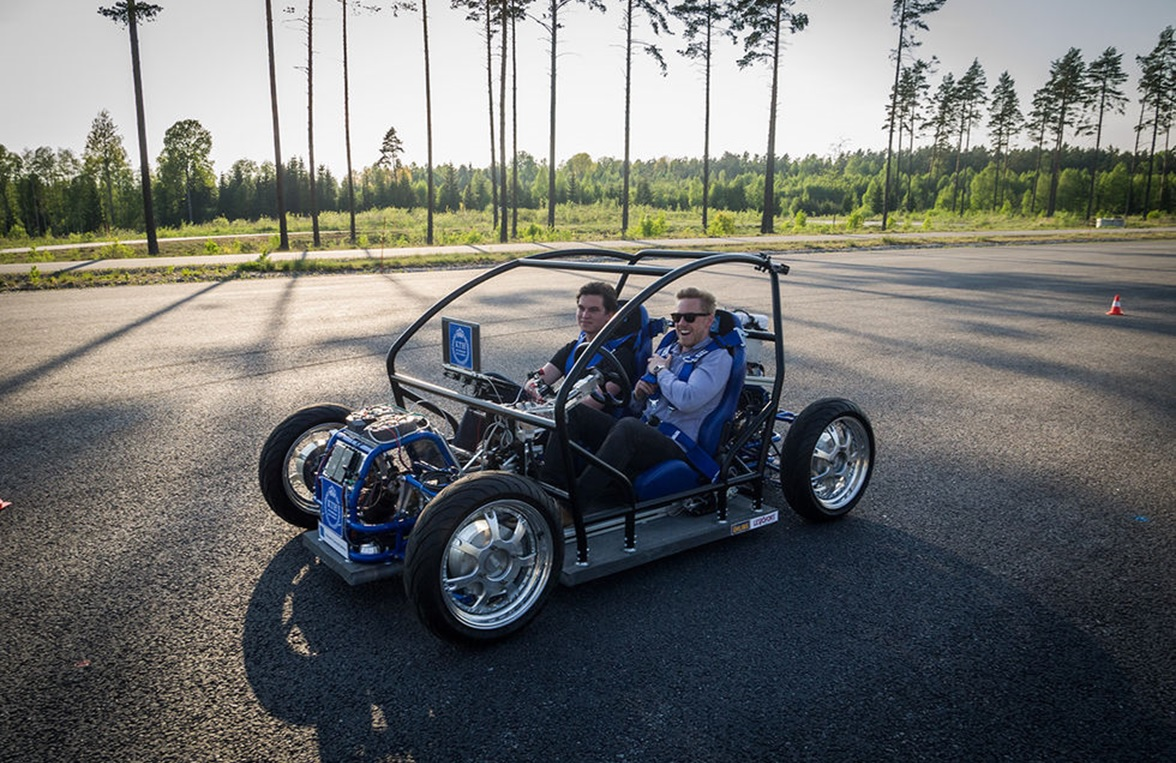
\includegraphics[width=\textwidth,trim={0 2.5cm 0 3.5cm},clip]{RCV.jpg}
\caption[Research Concept Vehicle of the ITRL]{Research Concept Vehicle of the Integrated Transport Research Lab}
\label{fig:RCV}
\end{figure}

% PATH PLANNING
\chapter{Path Planning}
\label{ch:pathPlanning}
This section will present and discuss a variety of different planning techniques, many of which will not only be applicable to path planning, but have much more general capabilities in solving problems that can be solved by planning.

\section{Planning}
First, one should understand the meaning of the word planning. Meriam Webster gives the following simple definition:``the act or process of making a plan to achieve or do something''. Given this general description it becomes obvious that one can mean very different things by saying the word planning. A person who wants to visit a friend and intents to use public transportation is planning. A politician that signs a bill and intents to persuade voters with this is planning. A navigation system in a car is planning when it is asked to calculate the route for a trip.

All these are obviously descriptions of planning. Planning in this thesis is understood as the search for a set of actions that transitions a given start state to a desired goal state. When planning is conducted by computers one has to do it programmatically, the result is thus a planning algorithm that usually returns the set of actions that transitions the start to the goal state (planning under uncertainty is not considered).

\section{Path}
If planning returns the set of actions that are necessary to transition from a start to a goal state, then one can say that a path would be the entire set of actions. More specifically a path in this thesis is the set of actions that move a vehicle from a current start state to a desired goal state through the Euclidean two dimensional plane.

\section{Basic Problem}
The problem addressed in this thesis shall be further specified and a general formulation be established. The robot is the only moving object in the world. The dynamics of the robot are not considered, hence removing any time dependencies. As collisions shall not occur they will not be modelled either.

Based on these simplifications the basic problem can be described as follows:
\begin{itemize}
\item $\calA \subset \calW$, the robot, is a single moving rigid object in world $\calW$ represented in the Euclidean space as $\R^2$
\item $\calO \subset \calW$, the obstacles, are stationary rigid objects in $\calW$
\item geometry, position and orientation of $\calA$ and $\calO$ are known a priori
\item \textbf{Problem:} given a start and goal pose of $\calA \subset \calW$, plan a path $\calP \subset \calW$ denoting the set of poses so that $\calA(p) \cap \calO = \emptyset$ for any pose  $p \in \calP$ along the path from start to goal, terminate if a path has been found report if no such path exists
\end{itemize}

\cite{Latombe.1991} \cite{LaValle.2006}

\section{Configuration Space}
In the literature of motion planning the concept of the configuration space has been well established, as it facilitates the formulation of path planning problems, presenting various concepts with an underlying scheme yielding great expressive power \cite{LaValle.2006} \cite{Latombe.1991}. Configuration spaces have been extensively used by Lozano-P\'{e}rez in the 80s for the description of spatial planning problems, e.g. the search for an appropriate space to place an object or the search for a path of an object in an unstructured environment with obstacles \cite{Latombe.1991}. The search for the appropriated placement and the path for an object, is a problem often encountered in design and manufacturing, where compactness needs to be achieved but maintainability shall not be sacrificed. The advantage of the configuration space representation is that it reduces the problem from a rigid body to a point and thus eases the search \cite{LozanoPerez.1983}.

Given the robot or agent $\calA \subset \calW$, where $\calW$ is the world as the two dimensional Euclidean space $\R^2$ with a fixed Cartesian coordinate frame $\calF_\calW$. In $\calW$ each possible configuration of $\calA$ can be described by $q$ of the form $(x,y,\theta)$ denoting a position along the $x$- and $y$-axis as well as an orientation in $\calF_\calW$ respectively. All possible configurations $q$ form the configuration space $\calC \subset \calW$. Attached to the robot $\calA$ is the frame $\calF_\calA$, so that $\calF_\calW(q) = \calF_\calA$, so that parts of the robot can be described relative to $\calA$ and not $\calW$. The configuration space of the robot can be further divided in subsets $\calC_{obs}$ and $\calC_{free}$. The configuration space $\calC_{obs} \subset \calC$ describes the set of all $q$ where $\calA(q) \cup \calO \neq \emptyset$ and hence the robot is in collision. On contrast $\calC_{free} \subset \calC$ is the set of all safe configurations $q$, $\calA(q) \cup \calO = \emptyset$ \cite{Latombe.1991} \cite{LaValle.2006}.

Since the configuration space only considers the static case, the regions defined are not fully descriptive, once dynamics are considered as well. In order to incorporate dynamics, analog to $C$ the state space $X$ can be introduced, with $X = \calC$. In addition to $\calC$, $X$ allows the description of the dynamics of the robot so that with $f: x \to q$ a given state $x$ with $(x,y,\theta,\dot{x},\dot{y})$ can be mapped to $q$ as $(x,y,\theta)$. Describing this will add another subset $X_{ric} \to \calC_{free}$ to $X$, the region of inevitable collision. This region describes all states that will lead to a collision due to robot's dynamics In $\calC$ this maps to $\calC_{free}$

\begin{figure}[h]
    \includegraphicsTex{MF.eps_tex}
    \caption{Configuration space of a robot}
    \label{fig:configurationSpace}
\end{figure}

\section{Popular Approaches}
As with most things, one can use a variety of different methods for path planning based on the requirements of the problem to be solved. The aim of the following is not to compare methods for path planning. Each has advantages and disadvantages, as discussed in many other places, but it should rather give the reade a quick overview over other solutions for the same problem. In the area of sampling-based methods Probabilistic Roadmaps (PRMs), Rapidly-exploring Random Trees (RRTs) as well as State Lattice planners are among the most popular to solve problems in higher dimensional state spaces.

Path planning as 

\begin{itemize}
    \item algorithms for discrete state spaces
    \item forward search in continuous space
    \item a non-linear optimization problem
\end{itemize}

\subsection{RRT}
Rapidly-exploring random trees were first introduced in the late 90s by Lavalle and Kuffner. The goal was to create an algorithm that could be applied to general nonholonomic as well as kinodynamic planning problems, which other randomized approaches such as the randomized potential field and probabilistic road map struggled with \cite{Lavalle.1998}. The basic structure is exemplified in the algorithm below.

A rapidly-exploring random tree (RRT) grows by repeatedly selecting a random state in a bounded region algorithm \algref{alg:RRT}{alg:RRTrandomState}. Starting from this random state the nearest neighbor is selected in line \ref{alg:RRTnearestNeighbor}. A new state is created in line \ref{alg:RRTnewState} by using an appropriate control action, line \ref{alg:RRTcontrolAction}. During this phase it needs to be ensured that the resulting edge will be collision free. Finally in line \ref{alg:RRTaddVertex} and \ref{alg:RRTaddEdge} the tree is being grown by adding the new state and the connecting edge. Using this approach the tree explorers the state space in a rapid and uniform manner as it probabilistically grows away from its root node \ref{fig:RRT} expanding towards larger Voronoi regions due to its randomization. Inherent to their nature RRTs are non guided and hence non optimal \cite{Lavalle.1999}. An RRT can however be biased by changing the probability distribution. Sampling in the goal region, allows for much faster convergence. Another approach is to include a measure that takes the path costs into account. Urmson presents a heuristically-guided RRT where the probability distribution takes the size of the Voronoi region into account as well as the quality of the path so far \cite{Urmson.2003}.

\begin{algorithm}
    \caption{Rapidly-exploring Random Tree}\label{alg:RRT}
    \begin{algorithmic}[1]
        \Require $x_s \cap x_g \in X_{free}$
        \State $T.init(x_s)$
        \While{$x_{new} \neq x_g$}
            \State $x_{rnd} \gets randomState()$ \label{alg:RRTrandomState}
            \State $x_{ngh} \gets nearestNeighbor(x_{rnd})$ \label{alg:RRTnearestNeighbor}
            \State $u \gets controlAction(x_{rnd}, x_{ngh})$ \label{alg:RRTcontrolAction}
            \State $x_{new} \gets newState(x_{rnd}, x_{ngh}, u)$ \label{alg:RRTnewState}
            \State $T.addVertex(x_{new})$ \label{alg:RRTaddVertex}
            \State $T.addEdge(x_{ngh}, x_{new}, u)$ \label{alg:RRTaddEdge}
        \EndWhile
        \State \textbf{return} $T$
    \end{algorithmic}
\end{algorithm}

\begin{figure}[h]
    \includegraphicsTex{MF.eps_tex}
    \caption{Rapidly-exploring random tree biased towards unexplored areas}
    \label{fig:RRT}
\end{figure}

\subsection{Potential Fields}
Potential Fields were originally used as an online collision avoidance measure for static as well as moving obstacles using the artificial potential field concept to make the collision avoidance part of lower level of control, decreasing response time. The idea behind the artificial potential field approach can be summarized, with the robot moving in a field of forces. The goal position is an attractive, while an obstacle creates a repulsive pole \cite{Khatib.1986}. The shape of the artificial potential field $U$ represents the layout of the configuration space. Path planning is conducted in an sequential. In each step the artificial force $\vec{F}(q) = -\vec{\triangledown}U(q)$ acting on the robot's current configuration will create a path increment towards this direction.

As obstacle avoidance was the original goal, potential fields come with the risk of not being able to reach the goal as the robot might get stuck in local minima. To work around this inherent characteristic one can try to formulate the potential function without local minima or incorporate techniques that allow the escape from the same \cite{Latombe.1991}.

\begin{figure}[h]
    \includegraphicsTex{MF.eps_tex}
    \caption{Potential Fields}
    \label{fig:potentialFields}
\end{figure}

\subsection{Approximate Cell Decomposition}
Path planning with approximate cell decomposition can be traced back to Brooks and Lozano-Peréz in the mid 80s. The basic idea is that the configuration space is divided into rectangles with edges parallel to the axes of the space. The resulting cells will be either free, occupied or mixed, depending on the configuration space of the obstacles intersecting with the respective rectangle or not, see \ref{fig:cellDecomposition}. The search for a path is conducted by finding a set of connected and free cells that include the start as well as the goal configuration \cite{Brooks.1985}. Applicable graph search algorithms are explained in more detail in chapter \ref{ch:graphSearch}.

This approach does not represent the free space exactly, hence a conservative approach must be taken in order to avoid faulty planning. Decomposing the cells in this way, although not exact, in general allows for planning methods that are easier to implement in comparison to exact cell decomposition \cite{Latombe.1991}

\begin{figure}[h]
    \includegraphicsTex{MF.eps_tex}
    \caption{Approximate Cell Decomposition}
    \label{fig:cellDecomposition}
\end{figure}

\section{Differential/Kinematic Constraints}
This section focuses on the differential constraints of a car-like robot. Most of the time these differential constraints are inherent to the kinematics and dynamics of the robot itself. These constraints need to be taken into account at some point, ideally during the actual path planning process ensuring the path matching the robot's constraints. In case that considering the constraints during the planning process is infeasible one could also unload this task on the controller, which given the constraints will not be an easy task either \cite{LaValle.2006}.

Even though a car can reach any position and orientation in the Euclidean plane, it cannot translate or rotate freely. A car can move forward as well as backward, but it cannot move sideways. Thi means that there are less possible actions than degrees of freedom, systems such as this are called underactuated, its configuration space is thus $\calC = \R^2 \times \S^1$, with a configuration as $q = (x,y,\theta)$ \cite{LaValle.2006}. A common case for drivers of cars is to parallel park, in order to achieve a configuration $q_1$ that is parallel to $q_0$ it is necessary for a car to at least rotate and translate the same goes for a third configuration $q_2$ that has the same position but different orientation than $q_0$ \cite{Latombe.1991}.

\begin{figure}[h]
    \includegraphicsTex{MF.eps_tex}
    \caption{Kinematic Constraints of a car-like robot}
    \label{fig:kinematicConstraints}
\end{figure}

\subsection{Reeds-Shepp Car}

\subsection{Dubins Car}

% COLLISION DETECTION
\chapter{Collision Detection}
Collision detection is a basic geometric operation that is applicable for many applications such as computer games, robotics and engineering simulations \cite{Ericson.2005} \cite{Ponamgi.1997} \cite{Chazelle.1987} . While some hard to model and computational intense planning approaches produce collision free paths by nature, others such as the ones introduced in chapter \ref{ch:pathPlanning}, require explicit collision checking along the paths they produce \cite{LaValle.2006}. Collision detection as a whole is concerned with the \emph{if}, \emph{when} and \emph{where} two objects collide \cite{Ericson.2005}. The focuses in the following is primarily on the \emph{if}. Another distinction can be made, with regard to discrete or continuous checking. While static collision detection is computationally much cheaper, it comes at the risk of tunneling, where both objects might pass each other from one time step to the next and the collision goes undetected \cite{Ericson.2005}.

A path $\calP$ produced by a motion planning algorithm needs to be collision free based on the information provided, hence $\calP \subset \calC_{free}$. If the environment of the robot changes, so that $\calP \cup \calC_{obs} \neq \emptyset$ a new path needs to be computed. Whether it is beneficial to recompute paths on every update of the environment or only perform collision checking for the previous path given the change in the environment depends on the specific case.

Collision detection can be conducted in a great variety of ways. The important thing to consider is the computational cost for checking whether $q \in \calP \land q \notin \calC_{obs}$ is true for a given configuration $q$, which can be seen as a logical predicate. As a path can only be considered safe, if its entirety of states is collision free, collision detection needs to be conducted along the entire length of the same.

While the use of the configuration space is beneficial due to its expressive power and verbosity it might not be useful during the actual collision detection \cite{LaValle.2006}

\begin{figure}[h]
    \includegraphicsTex{MF.eps_tex}
    \caption{Collision Detection}
    \label{fig:collisionDetection}
\end{figure}

\section{Hierarchical Methods}
Hierarchical methods break up a larger complicated convex bodies into a tree. The vertices of the the tree represent a bounding region containing a subset of the body as depicted in \Fref{fig:boundingRegions}.

Lavalle defines two criteria for the choice of appropriate bounding regions

\begin{itemize}
	\item The region should fit the intended body points as tightly as possible.
	\item The intersection test for two regions should be as efficient as possible.
\end{itemize}

A bounding box \cite{Ericson.2005} 

\begin{figure}[h]
    \includegraphicsTex{MF.eps_tex}
    \caption{Bounding regions}
    \label{fig:boundingRegions}
\end{figure}

\section{Spatial Occupancy Enumeration}
Spatial occupancy enumeration stores an exhaustive array of elements occupied by the respective body. In $\R^2$ these might be squares, in $\R^3$ cubes. This approach offers a trivial collision check that can be conducted rapidly. Enumerative schemes have the disadvantage that the respective spatial occupancy needs to be computed for each point of a given path \cite{Hayward.1986}. This problem can be avoided by discretion of the orientation values, so that the spatial occupancy enumeration can be stored in a lookup table.

\begin{figure}[h]
    \includegraphicsTex{MF.eps_tex}
    \caption{Spatial Occupancy Enumeration}
    \label{fig:spatialOccupancyEnumeration}
\end{figure}

% GRAPH SEARCH
\chapter{Graph Search}
\label{chap:graphSearch}
This chapter explains the basic theory necessary to understand graphs and the terminology associated with it. The later part of the chapter focuses on elaborating different graph search algorithms that are fundamental to understanding the implementation of the search algorithm in this thesis.

\section{Fundamentals}
A graph such as the one depicted in \fref{fig:graph} consists of vertices $V$ as well as edges $E$. With $G$ being a graph $V = V(G)$, is the set of vertices of the graph and $E = E(G)$, the set of Edges. Edges connect vertices of a graph. An edge of a graph can be described by ${x,y}$, as it connects the vertices $x$ and $y$. Edges that have at least one vertex in common are considered adjacent. \cite{Bollobas.1979}

Graphs can be either directed or undirected. A directed graph has unidirectional, a undirected graph bidirectional edges. In the following the word nodes and vertices might be used interchangeably.

\begin{figure}[h]
    \includegraphicsTex{MF.eps_tex}
    \caption{Graph theory explanation}
    \label{fig:graph}
\end{figure}

\subsection{State Space of a Graph}
While the chapter is termed graph search one has to understand that this term can be seen as the search for a set of actions that changes the state of an object from an initial state to a desired goal state. Given this general description graph search algorithms can be applied to a great variety of problems from motion planning to artificial intelligence \cite{LaValle.2006}.

The following definition constitutes a general description of the state space of a graph, it is borrowed from Lavalle's famous book titled \emph{Planning Algorithms}. 

\begin{enumerate}
    \item A nonempty \textit{state space} $x \in X$, which is finite or countably infinite set of \textit{states}.
    \item For each \textit{state} $x \in X$, a finite action space $U(x)$.
    \item A \textit{state transition function f} that produces a state $f(x,u) \in X$ for every $x \in X$ and $u \in U(x)$. The \textit{state transition equation} is derived from $f$ as $x' = f(x,u)$.
    \item An \textit{initial state} $x_s \in X$.
    \item A \textit{goal set} $X_G \subset X$.
\end{enumerate}

The vertices $V$ of the graph $G$ can be considered the state space $X$ of the $G$. Thus, each vertex holds information pertaining to a specific state. The edges $E$ are best represented by the action space $U$. Where an edge $u \in U(x)$ transitions a state $x \in X$ to a state $x' \in X$ with the state transition function $f(x,u)$.

\subsection{Open and Closed Lists}
For the explanation of the following algorithms two types of lists need special attention. On the one side there is the open list $O$, representing the set of the search frontier, the vertices, that have not yet been expanded, but have an adjacent vertex that has been expanded, hence any vertex $v_i \in O$ is part of the frontier. On the other side there is the closed list $C$, representing the set of vertices that have already been expanded.

\subsubsection{Priority Queues}
% Lavalle General Forward Search
Depending on the algorithm these lists need to implemented as a priority queue. A priority queue is a data structure that sorts a set by a key either from large to small or vice versa. The following operations are supported by the basic priority queue. All these actions maintain the order of the queue \cite{Skiena.2008}.

\begin{itemize}
    \item insertion of a given item with a given key
    \item find the minimum of the keys of the items in the queue
    \item delete the item with the minimum key from the queue
\end{itemize}

The type of queue chosen has a considerable impact on the time complexity for the operations mentioned above. When implementing a queue it is recommended to take this into consideration, as a more complex queue might yield considerable better performance, especially when operating on larger sets of data. While C++ implements a basic priority queue in the \emph{std} name space \url{http://en.cppreference.com/w/cpp/container/priority_queue} other more advanced queues (Binomial, Fibonacci, etc.) can be used with \emph{Boost} \url{http://www.boost.org/doc/libs/1_60_0/doc/html/heap.html}

\subsection{Optimality}
One of the great advantages of graph search algorithms compared to other approaches for path planning is that many algorithms are proven to be optimal. Bellman's principle of optimality reads below.
\begin{quotation}
    \noindent \emph{An optimal policy has the property that whatever the initial state and initial decision are, the remaining decisions must constitute an optimal policy with regard to the state resulting from the first decision.} \cite{Bellman.2003}
\end{quotation}

In essence any optimal solution for a problem that requires a sequence of decisions can only consist of optimal sub-solutions.

\begin{lemma}
    Given a weighted, directed graph $G = (V,E)$ with a cost function $g$: $E \rightarrow \mathbb{R}$ let $p = \{v_0, v_1,\ldots, v_k\}$ be a shortest path from vertex $v_0$ to vertex $v_k$ and, for any $i$ and $j$ such that $0 \leq i \leq j \leq k$, let $p_{ij} = \{v_i, v_{i+1},\ldots, v_j\}$ be the sub path of $p$ from vertex $v_i$ to vertex $v_j$. Then, $p_{ij}$ is a shortest path from $v_i$ to $v_j$.
\end{lemma}
 
\begin{proof}
    If we decompose the path $p$ into $v_0 \xrightarrow{p_{0i}} v_i \xrightarrow{p_{ij}} v_j \xrightarrow{p_{jk}} v_k$, then we have that $g(p) = g(p_{0i}) + g(p_{ij}) + g(p_{jk})$. Now, assume that there is a path $p'_{ij}$ from $v_i$ to $v_j$ with cost $g(p'_{ij}) < g(p_{ij})$. Then, $v_0 \xrightarrow{p_{0i}} v_i \xrightarrow{p'_{ij}} v_j \xrightarrow{p_{jk}}$ is a path from $v_0$ to $v_k$, that has a lesser cost $g(p_{0i}) + g(p'_{ij}) + g(p_{jk})$ than $g(p)$, which contradicts the assumption that $p$ is the shortest path from $v_0$ to $v_k$. \cite{Cormen.2009}
\end{proof}

\subsection{Admissibility}
Algorithms that find optimal paths on non-negative graphs are considered admissible \cite{Hart.1968}.

\subsection{Heuristics}
In order to find an optimal path the search needs to be systematic. Various search algorithms differ most significantly in the way they expand vertices \cite{LaValle.2006}. To avoid wasteful search of unpromising regions of a graph the search must be as informed as possible, only expanding nodes that have the potential to belong to the optimal path. If the search uses information that leads to skipping the expansion of a specific node, hence failing to find the optimal path, admissibility is forfeited.

Heuristics are used as an aid for approximating a solution in order to address the limitations of processing power, in some cases drastically reducing the search space. A finite amount of time only allows for a finite number of calculations. Although this comes without a suprise it still is a major limitation to problems that grow exponentially with search depth. While searching a graph the search needs to decide which vertex to expand and which edge to take. Information that aims to answer this question is considered a heuristic. A heuristic might be based on some cost estimates between the current vertex and the goal vertex. \cite{Newell.1976} 

A heuristic is a function that provides the necessary information that allows the algorithm to converge faster towards the goal. Only an admissible heuristic can lead to optimal results \cite{Hart.1968}.

\section{Breadth First Search}
Breadth First Search (BFS) was first developed by Moore and published by Lee in 1961 \cite{Lee.1961}. The BFS algorithm works on unweighted graphs (graphs with equal edge costs). In the original paper BFS is described by the author as ``a computer model of waves expanding from a source under a form of straight-line geometry''. BFS traverses a graph layer by layer, all vertices with depth $k$ in the graph are visited before it proceeds to vertices with depth $k+1$.

BFS does not consider edge costs, but only the number of expansions and can hence only be used on non-weighted graphs. On these graphs however BFS is complete and optimal, although the time and memory complexity is high, as the search is not guided \cite{Lee.1961,LaValle.2006} .

BFS traverses all vertices $V$ in a graph $G$ until the algorithm terminates (e.g. due to meeting a goal condition). While the search progresses every vertex $x \in V$ changes its state from undiscovered to discovered. In order to trace the route discovered by BFS, a direction and hence a predecessor is assigned to each vertex. The start vertex will thus be the root of the resulting tree of successor. This is the key property that makes BFS a suitable candidate to solve shortest path problems \cite{Skiena.2008}. \Fref[plain]{alg:BFS} depicts the structure of the search.

\begin{algorithm}
    \caption{Breadth First Search}\label{alg:BFS}
    \begin{algorithmic}[1]
        \Require $x_s \cap x_g \in X$
        \State $O = \emptyset$
        \State $C = \emptyset$
        \State $Pred(x_s) \gets null$
        \State $O.push(x_s)$
        \While{$O \neq \emptyset$}
            \State $x \gets$ O.pop()
            \State $C.push(x)$
                \For {$u \in U(x)$}
                    \State $x_{succ} \gets f(x,u)$
                    \If {$x_{succ} \notin C$}
                        \If {$x_{succ} \notin O$}
                            \State $Pred(x_{succ}) \gets x$
                            \If{$x_{succ} = x_g$}
                                \State \textbf{return} $x_{succ}$
                            \EndIf
                            \State $O.push(x_{succ})$
                        \EndIf
                    \EndIf
                \EndFor
        \EndWhile
        \State \textbf{return} null
    \end{algorithmic}
\end{algorithm}

\section{Dijkstra's or Uniform-Cost Search}
While Breadth First Search delivers optimal solutions to the discrete path planning problem it does not consider edge cost and is hence in its original form only applicable to uniform cost graphs. Dijkstra's search algorithm can be seen somewhat of a refinement, even though first published two years earlier than BFS, in 1959. This chapter is also called \emph{Uniform-Cost Search} as people such as Felner have pointed out that the original Dijkstra's algorithm was much closer to UCS than it is often conveyed in today's textbooks \cite{Felner.2011}. In his original paper Dijkstra indirectly refers to Bellman's principle of optimality, which is a needed proof for the algorithm being optimal.

Dijkstra's algorithm begins to divide all vertices into three sets, the closed set $C$, the open set $O$ (implemented as a priority queue) as well as the remaining vertices. At the beginning $C$ and $O$ are the empty sets. After this the algorithm starts as depicted in \fref{alg:Dijkstra} \cite{Dijkstra.1959}. First the start vertex $x_s$ gets transferred to the open set. Next the while loop is entered, line \ref{alg:DijkstraWhile}, which either returns the goal vertex (line \ref{alg:DijkstraSolution}) or null if the $O$ is the empty set. When a vertex gets expanded it is removed from $O$ and added to $C$. Afterwards all edges connected to the vertex are evaluated and the vertexes they connect to. If any of these vertexes are not in $C$ then we calculate the cost so far the same $g(x') = g(x) + l(x,u)$. Where $g(x)$ represents the cost-so-far for the vertex $x$ from the start vertex and $l(x,u)$ the cost for the state transition from $x$ to $x'$ given the action $u$. If the resulting cost is lower than the current cost to reach that vertex or that vertex is not an element of $O$, the predecessor and the cost for that vertex will be set and the position in the priority queue will be decreased or it will added to $O$ respectively. \cite{Dijkstra.1959,LaValle.2006,Cormen.2009} 

\begin{algorithm}
    \caption{Dijkstra's Search}\label{alg:Dijkstra}
    \begin{algorithmic}[1]
        \Require $x_s \cap x_g \in X$
        \State $O = \emptyset$
        \State $C = \emptyset$
        \State $Pred(x_s) \gets null$
        \State $O.push(x_s)$
        \While{$O \neq \emptyset$} \label{alg:DijkstraWhile}
            \State $x \gets$ O.popMin()
            \State $C.push(x)$
            \If{$x = x_g$}
                \State \textbf{return} $x$ \label{alg:DijkstraSolution}
            \Else
                \For {$u \in U(x)$}
                \State $x_{succ} \gets f(x,u)$
                    \If {$x_{succ} \notin C$}
                        \State $g \gets g(x) + l(x,u)$
                        \If {$x_{succ} \notin O$ \textbf{or} $g < g(x_{succ})$}
                            \State $Pred(x_{succ}) \gets x$
                            \State $g(x_{succ}) \gets g$
                            \If {$x_{succ} \notin O$}
                                \State $O.push(x_{succ})$
                            \Else
                                \State $O.decreaseKey(x_{succ})$
                            \EndIf
                        \EndIf
                    \EndIf
                \EndFor
            \EndIf
        \EndWhile
        \State \textbf{return} null
    \end{algorithmic}
\end{algorithm}

\section{A* Search}
If one thinks of Dijkstra's search as a refinement of BFS then A* Search can be seen as a refinement of Dijkstra's work. While Dijkstra associated a cost-so-far $g$ with each vertex of a graph to determine the next vertex to expand, A* enhances the algorithm by the use of a heuristic, allowing for much more rapid convergence under certain conditions, while still ensuring its optimality \cite{Hart.1968}. The heuristic $h(x)$ is the cost-to-come, based on an estimate of the cost from state $x$ to the goal state $x_g$. Just as Dijkstra's algorithm A* also starts with $O$ and $C$ being the open and closed list respectively.

\begin{algorithm}
    \caption{A* Search}\label{alg:A*}
    \begin{algorithmic}[1]
        \Require $x_s \cap x_g \in X$
        \State $O = \emptyset$
        \State $C = \emptyset$
        \State $Pred(x_s) \gets null$
        \State $O.push(x_s)$
        \While{$O \neq \emptyset$}
            \State $x \gets$ O.popMin()
            \State $C.push(x)$
            \If{$x = x_g$}
                \State \textbf{return} $x$
            \Else
                \For {$u \in U(x)$}
                \State $x_{succ} \gets f(x,u)$
                    \If {$x_{succ} \notin C$}
                        \State $g \gets g(x) + l(x,u)$
                        \If {$x_{succ} \notin O$ \textbf{or} $g < g(x_{succ})$}
                            \State $Pred(x_{succ}) \gets x$
                            \State $g(x_{succ}) \gets g$
                            \State $f(x_{succ}) \gets g(x_{succ}) + h(x_{succ})$
                            \If {$x_{succ} \notin O$}
                                \State $O.push(x_{succ})$
                            \Else
                                \State $O.decreaseKey(x_{succ})$
                            \EndIf
                        \EndIf
                    \EndIf
                \EndFor
            \EndIf
        \EndWhile
        \State \textbf{return} null
    \end{algorithmic}
\end{algorithm}

\newpage
\section{Hybrid A* Search}
The hybrid A* algorithm behaves similar to the A* algorithm. The key difference is, that state transitions happen in continuous rather than discrete space. The search starts by defining the empty sets $O$ and $C$, as well as by setting the predecessor state of the start state to $null$ and pushing the start state on the open list algorithm \algref{HA*}{HA*start}.

At line \ref{HA*while} the while loop starts, which only terminates if the open list is empty or the goal state has been reached line \ref{HA*solution}.

\paragraph{Notations}
\begin{itemize}
    \item start state $x_s \in X$
    \item goal state $x_g \in X$
    \item open list, implemented as priority queue $O$
    \item closed list $C$
    \item cost so far $g(x,x_s)$
    \item cost to go $h(x,x_g)$
    \item total estimated cost $f(x) = g(x,x_s) + h(x,x_g)$
\end{itemize}

\begin{algorithm}
    \caption{Hybrid A* Search}\label{HA*}
    \begin{algorithmic}[1]
        \Function{roundState}{$x$}
            \State $x.Pos_X = \max\{m\in\mathbb{Z}\mid m\le x.Pos_X\}$
            \State $x.Pos_Y = \max\{m\in\mathbb{Z}\mid m\le x.Pos_Y\}$
            \State $x.Ang_\theta\ =\max\{m\in\mathbb{Z}\mid m\le x.Ang_\theta\}$
            \State \textbf{return} $x$
        \EndFunction
        \Statex
        \Function{exists}{$x_{succ}$,$O$}
            \If{$\{ x \in O \mid roundState(x) = roundState(x_{succ})\} \neq \emptyset$}
                \State \textbf{return} $f(x)$
            \Else
                \State \textbf{return} 0
            \EndIf
        \EndFunction
        \Statex
        \Require $x_s \cap x_g \in X$
        \State $O = \emptyset$ \label{HA*start}
        \State $C = \emptyset$
        \State $Pred(x_s) \gets null$
        \State $O.push(x_s)$
        \While{$O \neq \emptyset$} \label{HA*while}
            \State $x \gets$ O.popMin()
            \State $C.push(x)$
            \If{$roundState(x) = roundState(x_g)$}
                \State \textbf{return} $x$ \label{HA*solution}
            \Else
                \For {$u \in U(x)$}
                \State $x_{succ} \gets f(x,u)$
                    \If {$x_{succ} \notin C$}
                        \State $f \gets g(x) + l(x,u) + h(x_{succ})$
                        \If {$exists(x_{succ},O) = 0$ \textbf{or} $f < exists(x_{succ},O)$}
                            \State $Pred(x_{succ}) \gets x$
                            \State $g(x_{succ}) \gets g$
                            \State $f(x_{succ}) \gets g(x_{succ}) + h(x_{succ})$
                            \If {$x_{succ} \notin O$}
                                \State $O.push(x_{succ})$
                            \Else
                                \State $O.decreaseKey(x_{succ})$
                            \EndIf
                        \EndIf
                    \EndIf
                \EndFor
            \EndIf
        \EndWhile
        \State \textbf{return} null
    \end{algorithmic}
\end{algorithm}

\part{Method, Implementation and Results}
% METHOD
\chapter{Method}
The second part of this thesis shall give an overview over the actual method used, its implementation as well as the results. This chapter will talk about the method used to solve the navigation problem.

\section{Hybrid A* Search}
As described in \fref{sec:HA} the hybrid A* (HA*) search expands vertices in continuous rather than discrete space. Even though it works in continuous space, HA* uses a discretized description of the world by pruning search branches that have similar leaf states. This is done in order to avoid growth of similar branches that add only very little to the solution, but vastly increase the size of the search graph.

A state is characterized by $\bldx = (x, y, \theta)$, where $x$ and $y$ denote the position and $\theta$ the heading of the vertex respectively. The action set $U$ for a given vertex $x$ can take any shape\footnote{An opposing method is to use a state lattice, where a large amount of motion primitives connect cells always in a predefined manner.}. In order to adhere to the constraints imposed by a non-holonomic vehicle, a vertex is expanded by one of three actions; maximum steering left, maximum steering right as well as no steering. Each of this control actions is applied for a certain amount of time, resulting in an arc of a circle with a lower bound turning radius based on the vehicle constraints. This will ensure that the resulting paths are always drivable, as the actual vehicle model is used to expand vertices, even though they might result in excessive steering actions.

HA* does not take the velocity of the vehicle into account, but based on the solution of HA* an appropriate velocity profile can easily be calculated.

To incorporate the heading of the vehicle a finite three dimensional cuboid, which represents all possible states of the vehicle is used. During the expansions of vertices with the actions $u \in U(x)$ new states are generated. If a new state falls into a grid cell that is already occupied with another vertex and the new vertex has a lower \textit{cost-so-far} the old vertex gets pruned (deleted). The search continues until a vertex reaches the goal grid cell, or all reachable cells have been reached and thus the open list is empty.

\subsection{Vertex Expansion and Branch Pruning}
The search starts with the current state of the vehicle, denoted as $x_s$. HA* will generate six successor vertices; three driving forward as well as three driving reverse, \Fref{fig:expansionPruning} depicts the expansion. The successors are generated by using arcs with the minimum turning radius of the vehicle\footnote{The arc length used for the expansion can be chosen arbitrarily, however a shorter length promises higher levels of resolution completeness, as the likelihood to reach each state is increasing.}. The cost for the state transition is based on the length of the arc. Additional costs are accrued for changing driving directions, driving in reverse; and turning, as opposed to going straight. The penalty for turning as well as driving in reverse are multiplicative (depend on portion of the path turning or reversing), while the penalty for the change of driving directions is constant.



For each successor the following actions will be executed. If the successor vertex reaches a cell of the three dimensional cuboid that is not part of the closed list (meaning that cell has not yet been expanded) the evaluation continues. If the cell is not part of the open list (meaning the cell has not been reached prior by any other vertex expansion) or the \textit{cost-so-far} from the predecessor vertex plus the cost for the vertex expansion to the successor reaching the cell is lower than the \textit{cost-so-far} of the vertex currently associated with that cell, then the new vertex will be assigned a pointer to its predecessor, the sum of the \textit{cost-so-far} from its predecessor plus the cost for the expansion will be assigned to its $g$-value and the \textit{cost-to-come} will be estimated using the heuristics and assigned to its $h$-value. If the a vertex with the same cell as the successor is on the closed or the open list and the successor's $g$-value is not lower, then the successor will be discarded, the branch will get pruned.

Under the assumption that the steering actions are either maximum steering right, no steering, or maximum steering left the arc length can be simply expressed as $r\abs{x_\theta- x'_\theta}$, $r$ being the minimum turning radius of the vehicle.

In case the arc length is shorter than the square root of the cell area, a vertex expansion can result in the successor arriving in the same cell. 
If this happens, it is insufficient to compare the vertices based on their \textit{cost-so-far} as the cost of the new vertex will always be higher. Thus the comparison is based on the total estimated cost for both vertices. Since the algorithm is using consistent heuristics this leads to the effect, that the optimistic estimate will make vertices that are closer to the goal more expensive\footnote{The total estimated cost of a vertex $x$ is $f(x) = g(x)+h(x)$ and the successor cost $f(x) = g(x) + l(x,u)  + h(x_{succ}) $ using a consistent heuristic implies $ h(x) \leq  l(x,u)  + h(x_{succ})$}, hence a tie breaker is added to the predecessor to account for the consistent nature of the heuristic.\Fref{alg:sameCellExpansion} illustrates this process. If the successor vertex is more expensive it will be discarded and the algorithm proceeds.

\begin{algorithm}
\caption{Same Cell Expansion}\label{alg:sameCellExpansion}
    \begin{algorithmic}[1]
                \For {$u \in U(x)$}
                \State $x_{succ} \gets f(x,u)$
                    \If {$\neg exists(x_{succ},C)$}
                        \If {$RoundState(x) = RoundState(x_{succ})$}
	                        \If {$ f(x_{succ}) > f(x_{x}) + tieBreaker$}
		                        \State \textbf{delete} $x_{succ}$
                        		 \State \textbf{continue}
        	                \EndIf            
            	                \State $Pred(x_{succ}) \gets x$
                	            \State $g(x_{succ}) \gets g$
                    	        \State $h(x_{succ}) \gets Heuristic(x_{succ}, x_g)$
                        	    \If {$\neg exists(x_{succ},O)$}
                            	    \State $O.push(x_{succ})$
                           		\Else
                                	\State $O.decreaseKey(x_{succ})$
                        \EndIf
                        \EndIf
                    \EndIf
                \EndFor
    \end{algorithmic}
\end{algorithm}

\begin{figure}[h]
    \includegraphicsTex{MF.eps_tex}
    \caption{Vertex expansion and pruning}
    \label{fig:expansionPruning}
\end{figure}

\subsection{Analytical Expansion}
The HA* planner sporadically calculates Dubins and Reeds Shepp curves from vertices currently being expanded to the goal. This is done partly as the exact continuous goal location is not reachable by the discretized control actions alone and in order to increase search speed. The calculated path is checked for collisions with the environment, if none exist the search terminates. In order to reduce computational load it is not beneficial to probe for these optimal point to point solutions from each vertex, but rather every n-th iteration (increasing the frequency while approaching the goal). Furthermore it is more reasonable to do so when approaching the goal or in a very obstacle sparse environment, as the likelihood for a collision is high otherwise, making this an expensive operation with little chance to payoff.

\subsection{Collision Checking}
While there are many ways to determine whether a configuration of the vehicle is collision free, $q \in \calC_{free}$. The spatial occupancy enumeration approach presented in \fref{sec:spatialOccupancyEnumeration} is used for collision checking. In order to make this a viable solution it is mandatory to precompute possible configurations of the vehicle and save these in a lookup table. The advantage of this approach is that the collision checking can be conducted rapidly in constant time for any configuration of the vehicle.

As the lookup can easily be translated to a specific two dimensional cell with integer coordinates for $x$ and $y$, only the different possible headings need to be taken into account. In order to compute spatial occupancy of a shape denoted by its corner points Bresenham's line algorithm can be used, but it does not correctly occupies all cells that the line between two points intersects with. For collision checking however, there needs to be certainty, thus a ray tracing algorithm described in \cite{Amanatides.2011} is used, that correctly marks all cells the line intersects with.

Once the basic bounding box is computed the lookup table gets filled with the spatial occupancy of the vehicle while rotating it with the $\theta$ discretization steps. In order to account for the hybrid nature of HA*, and the fact, that the vehicle, can reach any position within a cell, the spatial occupancy is also precomputed for 100 different positions within the grid cell.

\section{Heuristics}
While the goal is to produce drivable solutions that are approaching the optimum, it is important to make use of A* being an informed search, implementing heuristics allowing the algorithm converge quickly towards the solution. HA* is using estimates from two heuristics. As both of the heuristics are admissible the maximum of the two is chosen for any given state. The two heuristics capture very different parts of the problem; the constrained heuristic incorporates the restrictions of the vehicle, ignoring the environment, while the unconstrained heuristic disregards the vehicle's constraints and only accounts for obstacles.

\subsection{Constrained Heuristic}
The constrained heuristic takes the characteristics of the vehicle into account, while neglecting the environment. Suitable candidates are either Dubins or Reeds-Shepp curves. These curves introduced in \fref{sec:differentialConstraints} are the paths of minimal length with an upper bound curvature for the forward, and the forward as well as backward driving car respectively.

Since this heuristic takes the current heading as well as the turning radius into account it ensures, that the vehicle approaches the goal with the correct heading. This is especially important, when the car gets closer to the goal. For performance reasons this heuristic can be precomputed and stored in a lookup table. This is possible since it ignores obstacles and hence does not require any environment information. To precompute the heuristic estimate values the curves of minimal length are calculated in a discretized neighborhood of the goal.

Given that both Dubins as well as Reeds-Shepp curves are minimal, this heuristic is clearly admissible.

\subsection{Unconstrained Heuristic}
The unconstrained heuristic neglects the characteristics of the vehicle and only accounts for obstacles. The estimate is based on the shortest distance between the goal node and the vertex currently being expanded. This distance is determined using the standard A* search in two dimensions ($x,y$ position) with an Euclidean distance heuristic.
The two dimensional A* search uses the current vertex as the goal vertex, and the goal vertex of the HA* search as the start vertex. This is beneficial, since the closed list of the A* search stores all shortest distances $g(x)$ to the goal and can thus be used as a lookup table, instead of initiating a new search.

The unconstrained heuristic guides the vehicle away from dead ends and around u-shaped obstacles.

Since HA* can reach any point in a cell the unconstrained heuristic needs to be discounted by the absolute difference of the continuous coordinate of the current and the goal vertex.

\begin{figure}[h]
    \centering
    \begin{subfigure}[t]{0.45\textwidth}
        \includegraphicsTex{constrainedGood.pdf_tex}
        \caption{The constrained heuristic accounting for the goal heading.}
        \label{fig:constrainedGood}
    \end{subfigure}
    \hfill
    \begin{subfigure}[t]{0.45\textwidth}
        \includegraphicsTex{unconstrainedBad.pdf_tex}
        \caption{The unconstrained heuristic heavily underestimating the cost of the path, due to the wrong heading.}
        \label{fig:unconstrainedBad}
    \end{subfigure}
        \begin{subfigure}[t]{0.45\textwidth}
        \includegraphicsTex{constrainedBad.pdf_tex}
        \caption{The constrained heuristic heavily underestimating the cost of the path, due to ignoring obstacles.}
        \label{fig:constrainedBad}
    \end{subfigure}
    \hfill
    \begin{subfigure}[t]{0.45\textwidth}
        \includegraphicsTex{unconstrainedGood.pdf_tex}
        \caption{The unconstrained heuristic accounting for obstacles and dead ends.}
        \label{fig:unconstrainedGood}
    \end{subfigure}
    \caption{The constrained heuristic}
    \label{fig:heuristicComparison}
\end{figure}

\section{Collision Checking}

% PATH SMOOTHING
\section{Path Smoothing}
As the paths produced by the hybrid A* algorithm are drivable, but often are made up of unnecessary steering actions it is beneficial to post process the result with a smoother that attains a higher degree of comfort and safety \cite{Dolgov.2010}. For this purpose a gradient descent smoother is used that aims to minimize $P$ consisting of the following four terms with respect to the path.

\begin{equation}
P = P_{obs} + P_{cur} + P_{smo} + P_{vor}
\end{equation}

\subsection{Obstacle Term}

This term penalizes collisions with obstacles. For all vertices $\bldx_i$ where $|\bldx_i - \bldo_i| \leq d_{obs}^{\lor}$ the cost $P_{vor}$ is defined. It based on the the distance to the next obstacle.

\begin{equation}
P_{obs} = w_{obs} \displaystyle\sum_{i=1}^{N} \sigma_{obs}(|\bldx_i-\bldo_i|-d_{obs}^{\lor})
\end{equation}

Where $\bldx_i$ is the $x,y$-position of a vertex on the path, $\bldo_i$ the location of the closest obstacle to $\bldx_i$. $d_{obs}^{\lor}$ acts as a threshold for the the maximum distance obstacles can affect the cost of the path. In order to penalize heavier when getting close to obstacles $\sigma_{obs}$ is a quadratic penalty function. The obstacle weight $w_{obs}$ is used to influence the impact on the change of the path.

\paragraph{Gradient}

\begin{equation}
\frac{\partial \sigma_{obs}}{\partial \bldx_i} = \frac{2(|\bldx_i-\bldo_i|-d_{obs}^{\lor})\bldx_i-\bldo_i}{|\bldx_i-\bldo_i|}
\end{equation}

\subsection{Curvature Term}
In order to ensure driveabiliy the curvature term upper-bounds the instantaneous curvature of the path at every vertex. It is defined for $\frac{\Delta\phi_i}{|\Delta\bldx_i|} > \kappa_{max}$

\begin{equation}
P_{cur} = w_{cur} \displaystyle\sum_{i=1}^{N-1} \sigma_{cur}\left(\frac{\Delta\phi_i}{|\Delta\bldx_i|} - \kappa_{max}\right)
\end{equation}

The the displacement vector at the vertex $\bldx_i$ is defined as $\Delta\bldx_i= \bldx_i - \bldx_{i-1}$. The change in tangential angle at a vertex can be expressed by $\Delta\phi_i$ = $\cos^{-1}\frac{\bldx_{i}\cdot\bldx_{i+1}}{|\bldx_{i+1}||\bldx_{i+1}| }$.  The maximum allowable curvature is denoted by $\kappa_{max}$. Deviations from the maximum allowable curvature are penalized with a quadratic penalty function $\sigma_{cur}$. The curvature weight $w_{cur}$  controls the impact on the change of the path.

\paragraph{Gradients}

\begin{equation}
\frac{\partial \kappa_i}{\partial \bldx_i} = \frac{1}{|\Delta\bldx_i|}\frac{\partial\Delta\phi_i}{\partial\cos\Delta\phi_i}\frac{\partial\cos\Delta\phi_i}{\partial\bldx_i}-\frac{\Delta\phi_i}{{\Delta\bldx_i}^2}\frac{\partial\Delta\bldx_i}{\partial\bldx_i}
\end{equation}

\begin{equation}
\frac{\partial \kappa_i}{\partial \bldx_{i-1}} = \frac{1}{|\Delta\bldx_i|}\frac{\partial\Delta\phi_i}{\partial\cos\Delta\phi_i}\frac{\partial\cos\Delta\phi_i}{\partial\bldx_{i-1}}-\frac{\Delta\phi_i}{{\Delta\bldx_i}^2}\frac{\partial\Delta\bldx_i}{\partial\bldx_{i-1}}
\end{equation}

\begin{equation}
\frac{\partial \kappa_i}{\partial \bldx_{i+1}} = \frac{1}{|\Delta\bldx_i|}\frac{\partial\Delta\phi_i}{\partial\cos\Delta\phi_i}\frac{\partial\cos\Delta\phi_i}{\partial\bldx_{i+1}}
\end{equation}

\subsection{Smoothness Term}
The smoothness term evaluates the displacement vectors between vertices. The result is that it assigns cost to vertices that are unevenly spaced as well as change direction. $w_{smo}$ denotes the smoothness weight and hence the impact of the term on the change of the path.

\begin{equation}
P_{smo} = w_{smo} \displaystyle\sum_{i=1}^{N-1} (\Delta\bldx_{i+1} - \Delta\bldx_i)^2
\end{equation}

\subsection{Voronoi Term}
This term guides the path away from obstacles. For $d_{obs} \leq d_{vor}^{\lor}$ the cost $P_{vor}$ is defined. It is based on the position of the node in the Voronoi field.

\begin{equation}
P_{vor} = w_{vor} \displaystyle\sum_{i=1}^{N} \left(\frac{\alpha}{\alpha + d_{obs}(x,y)}\right)\left(\frac{d_{vor}(x,y)}{d_{obs} + d_{vor}(x,y)}\right)\left(\frac{(d_{obs}(x,y) - d_{vor}^{\lor})^2}{(d_{vor}^{\lor})^2}\right)
\end{equation}

The positive distance to the nearest obstacle is denoted by $d_{obs}$, $d_{edg}$ is the positive distance to the nearest edge of the GVD. $d_{vor}^{\lor}$ represents the maximum distance obstacles affect the Voronoi potential. $\alpha > 0$ controls the falloff rate of the field and $w_{vor}$, the Voronoi weight, influences the impact on the path.

\paragraph{Gradients}

\begin{equation}
\frac{\partial d_{obs}}{\partial \bldx_i} = \frac{\bldx_i-\bldo_i}{|\bldx_i-\bldo_i|}
\end{equation}

\begin{equation}
\frac{\partial d_{edg}}{\partial \bldx_i} =\frac{\bldx_i-\blde_i}{|\bldx_i-\blde_i|}
\end{equation}

\begin{equation}
\frac{\partial\rho_{vor}}{\partial d_{obs}} = \frac{\alpha d_{edg}\left(d_{obs}-d_{vor}^{\lor}\right)\left(\left(d_{edg}+2d_{vor}^{\lor}+\alpha\right) d_{obs}+\left(d_{vor}^{\lor}+2\alpha\right)d_{edg}+\alpha d_{vor}^{\lor}\right)}{{d_{vor}^{\lor}}^2\left(d_{obs}+\alpha\right)^2\left(d_{obs}+d_{edg}\right)^2}
\end{equation}

\begin{equation}
\frac{\partial\rho_{vor}}{\partial d_{edg}} =  \frac{\alpha d_{obs}\left(d_{obs}-d_{vor}^{\lor}\right)^2}{{d_{vor}^{\lor}}^2\left(d_{obs}+\alpha\right)\left(d_{edg}+d_{obs}\right)^2}
\end{equation}

\section{Path Analysis}

% IMPLEMENTATION
\chapter{Implementation}
The development of the algorithm is solely conducted in simulation and open-loop experiments.

Receiving a binary obstacle map as an input, the hybrid A* planner is able to plan a path from an initial state $x_s$ to a final state $x_g$ in a matter of milliseconds on medium grade consumer hardware (Intel Core i5-5200U 2.2GHz), making the planner a highly viable option for real world driving in unstructured environments.

%\begin{figure}[h]
%    \includegraphicsTex{MF.eps_tex}
%    \caption{Dijkstra's Algorithm, A* and hybrid A*}
%    \label{fig:searchComparison}
%\end{figure}

\section{Path Smoothing}

\section{Algorithm}

Under the assumption that the steering actions are either maximum steering right, no steering, or maximum steering left the arc length can be simply expressed as $r\abs{x_\theta- x'_\theta}$, $r$ being the minimum turning radius of the vehicle. 

Calculation of the new states $x'$, with the initial state $x$ consisting of :\\
$x_x, x_y, x_\theta$ the turning radius $r$, the turning angle $\theta$ and distance $d$ as well as the unit vector $e = \left(\begin{smallmatrix}0\\1\end{smallmatrix}\right)$
\begin{description}
  \item[left] \hfill \\
  $r_\theta = x_\theta + \frac{\pi}{2}$\\
  $x'_\theta = x_\theta + \theta$
  \item[right] \hfill \\
  $r_\theta = x_\theta - \frac{\pi}{2}$\\
  $x'_\theta = x_\theta - \theta$
  \item[left and right] \hfill\\
  $r_x = r(e_x\cos(r_\theta) - e_y\sin(r_\theta)) + x_x$\\
  $r_y = r(e_x\sin(r_\theta) - e_y\cos(r_\theta)) + x_y$\\
  $x'_x = (x_x-r_x)\cos\theta - (x_y-r_y)\sin\theta + r_x$\\
  $x'_y = (x_x-r_x)\sin\theta - (x_y-r_y)\cos\theta + r_y$
  \item[straight] \hfill \\
  $x'_x = x_x - d\sin(x_\theta)$\\
  $x'_y = x_y + d\cos(x_\theta)$
\end{description}

% RESULT AND ANALYSIS
\chapter{Results and Discussion}
For the test of the algorithm different scenarios have been chosen and simulations were conducted to test the efficiency and accuracy of the path planning. The scenarios chosen for the simulation describe common problems path planning algorithms need to be able to overcome in order to be usable for the navigation in unstructured environments. The problems are depicted in \Fref{fig:scenarioDeadEnd}, \Fref{fig:scenarioParkingStructure} and \Fref{fig:scenarioRandomObstacles}.

The scenarios shall test the algorithm for different scenarios.

\begin{figure}[h]
    \includegraphicsTex{scenarioDeadEnd.pdf_tex}
    \caption{The dead end scenario}
    \label{fig:scenarioDeadEnd}
\end{figure}

\begin{figure}[h]
    \includegraphicsTex{scenarioParkingStructure.pdf_tex}
    \caption{The parking structure scenario}
    \label{fig:scenarioParkingStructure}
\end{figure}

\begin{figure}[h]
    \includegraphicsTex{scenarioRandomObstacles.pdf_tex}
    \caption{The random obstacles scenario}
    \label{fig:scenarioRandomObstacles}
\end{figure}

\section{Results}

\subsection{Simulation Results}

\begin{figure}[h]
    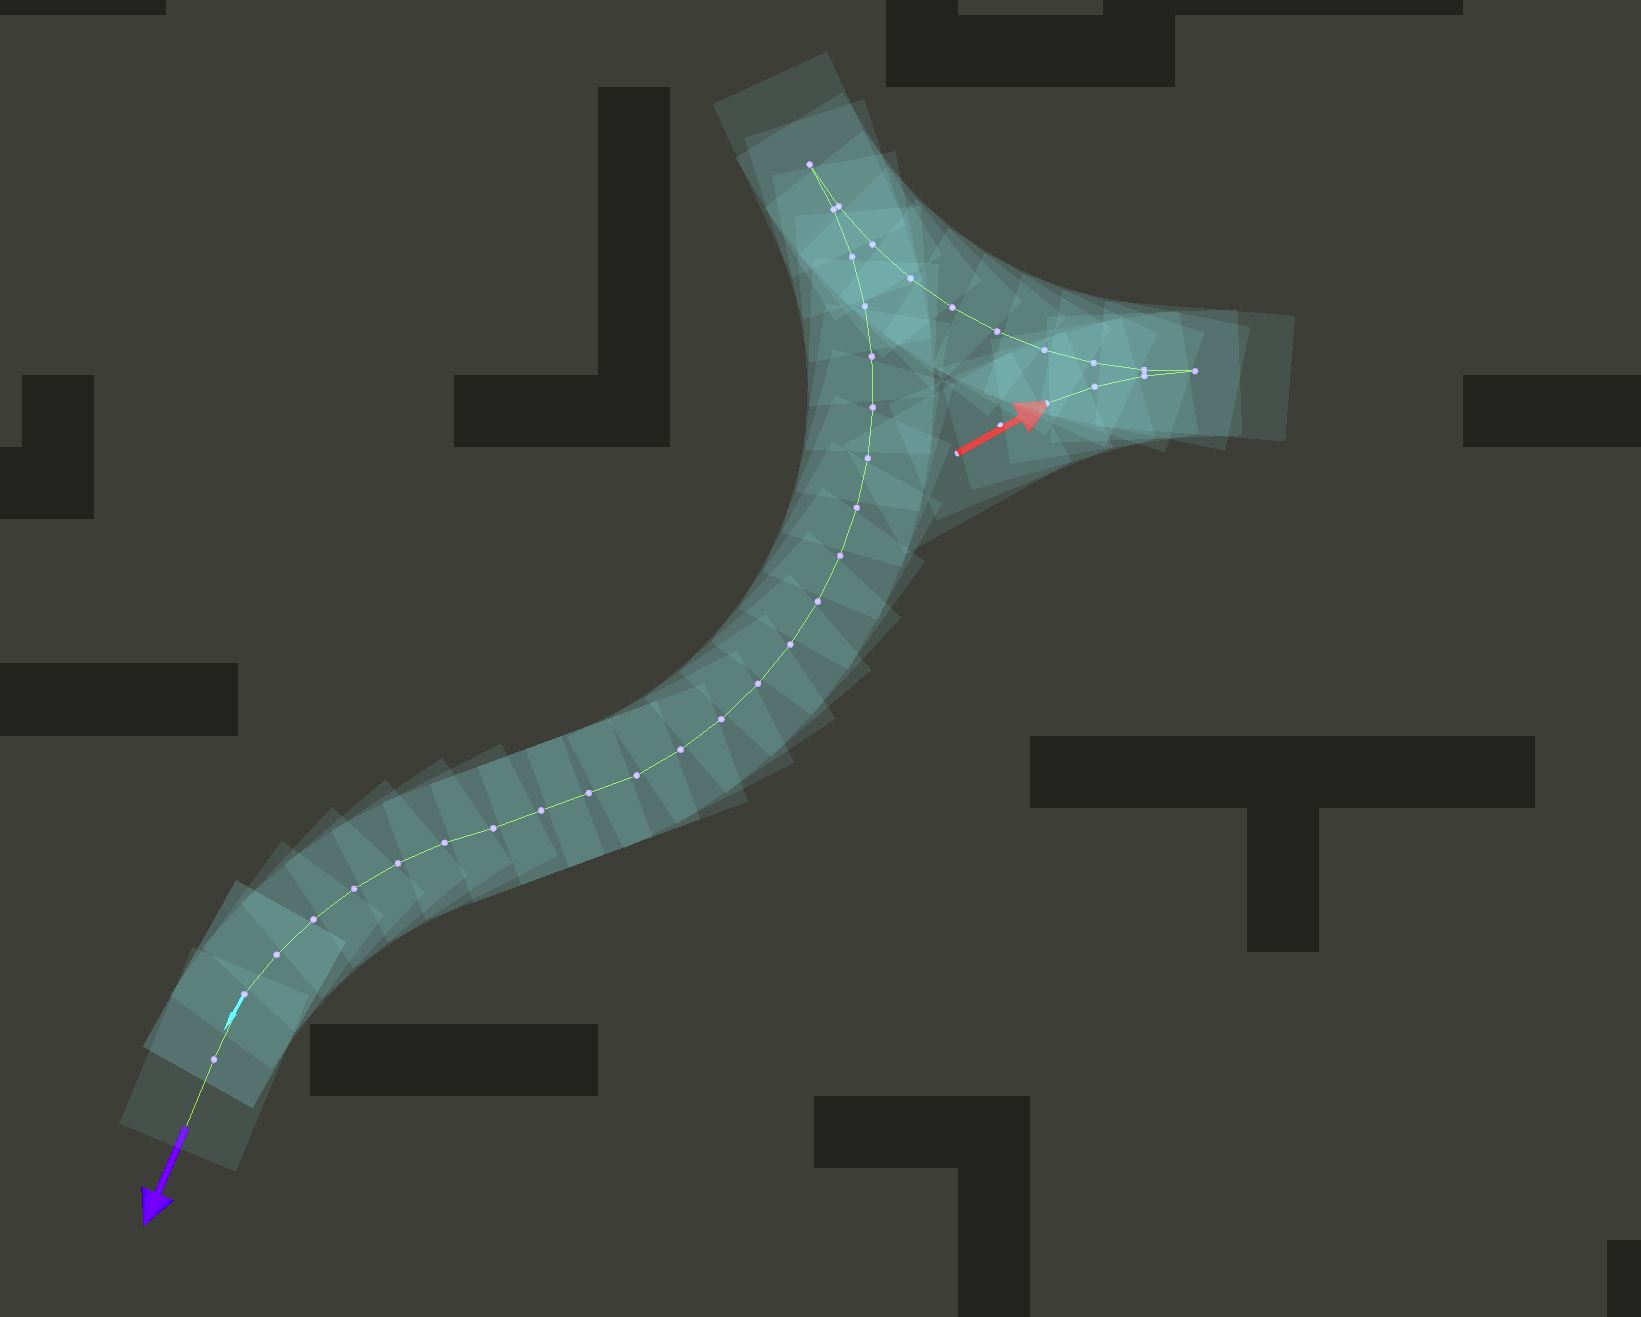
\includegraphics[width=\textwidth]{threePointTurn.png}
    \caption{Three point turn for change of directions}
    \label{fig:threePointTurn}
\end{figure}

\begin{figure}[h]
    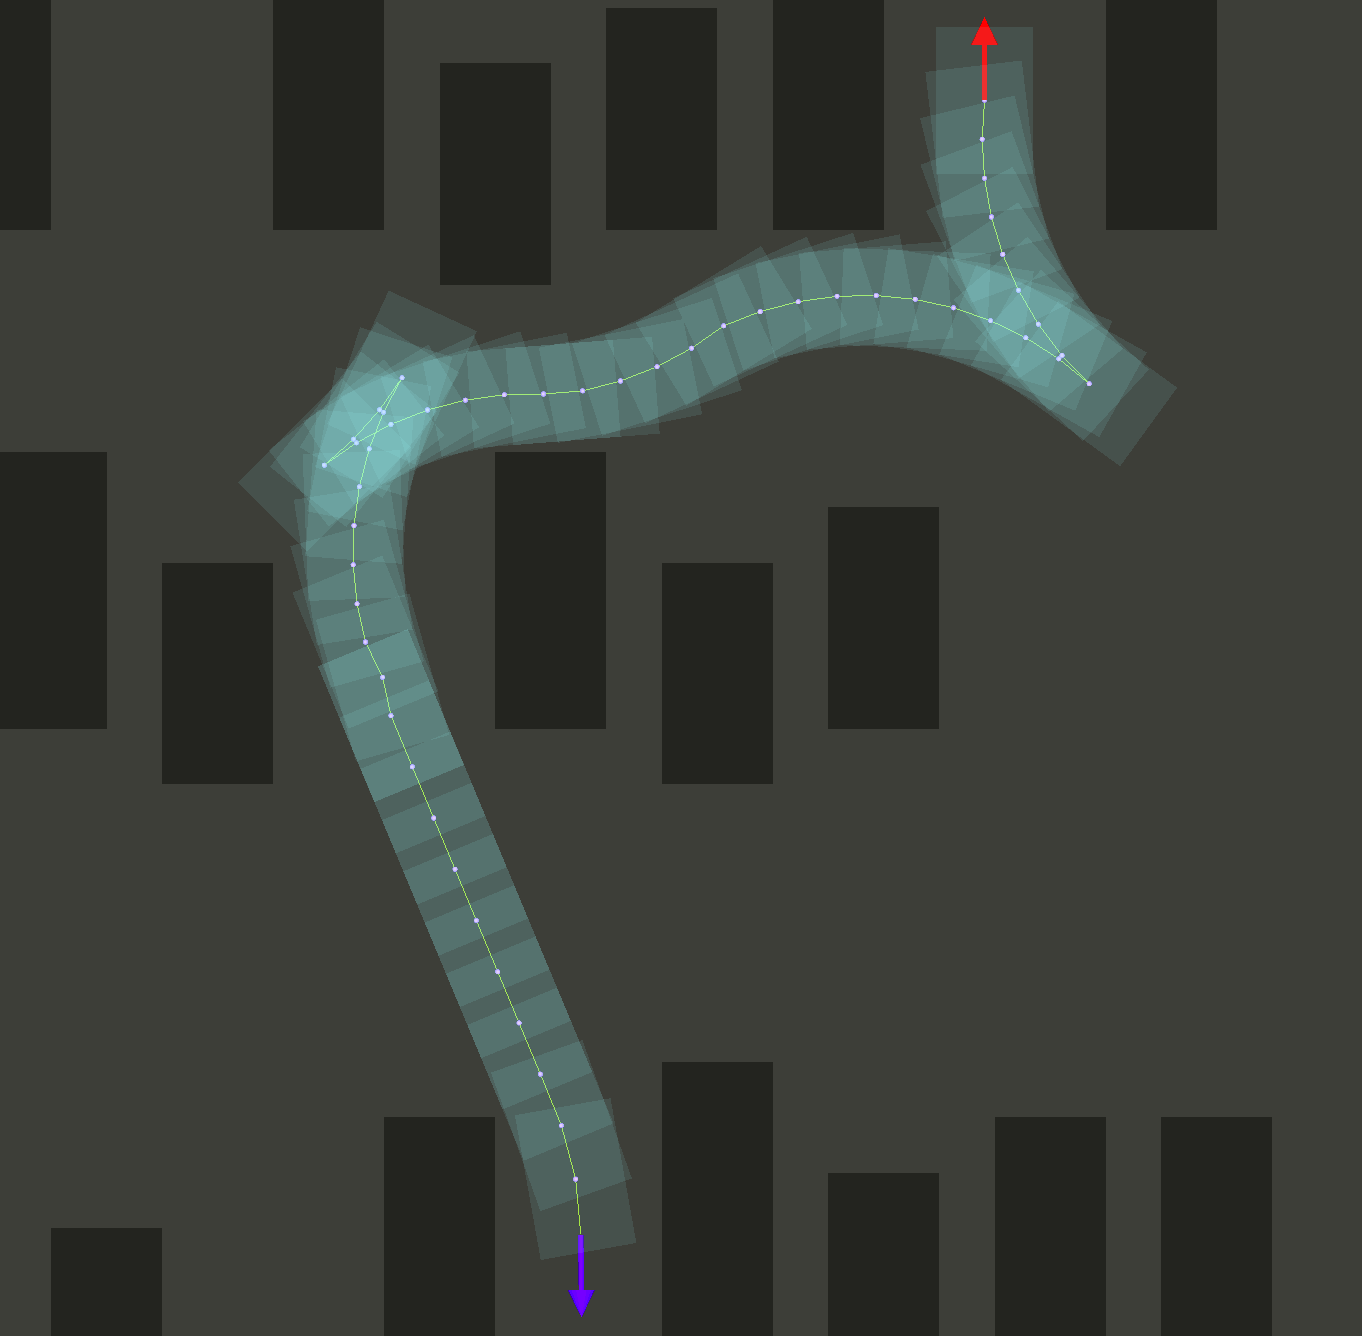
\includegraphics[width=\textwidth]{parking.png}
    \caption{Change of parking spot in a parking lot}
    \label{fig:parking}
\end{figure}

\subsection{Real-world Results}

\section{Analysis}

% CONCLUSION
\chapter{Conclusion}
While the research in the area of autonomous driving continuous to grow, the DARPA Grand Challenge and especially the Urban Challenge have marked important milestones, greatly propelling the development. Hence it is not astonishing that companies heavily engaged in autonomous driving, such as Alphabet (formerly Google) or Uber recruited a large part of past participants of these challenges.

Since there are many ways to solve navigation problems of this kind the choice might seem arbitrary. While the team from CMU and winner of the DUC used a lattice planner with D* \cite{Ferguson.2008b,Likhachev.2005}, the MIT team used an heavily modified version of RRT both for structured as well as unstructured driving \cite{Kuwata.2008}.

The hybrid A* algorithm is yet another approach. It is a fast planner used for planning in unstructured environments by the Standford team, developed by Dolgov, Thrun, Montemerlo (Google Self-Driving Cars), Diebel (Cedar Lake Ventures), participating with Junior in the DUC.
This thesis has analyzed HA* thoroughly and developed a very similar version for the KTH RCV in \texttt{C++} and ROS.

The resulting hybrid A* planner addresses the problem of finding a solution to the problem described in \fref{sec:problemDescription} properly. The planner models the non-holonomic nature of the vehicle in all stages of the process, vertex expansion, heuristic estimates, as well as path smoothing. Thus, the most important characteristic of the paths is given--they are driveable. 

The HA* planner solves a challenging problem in an elegant manner. HA* is fast, as it reduces the search space with the help of well informed heuristics, allowing it to converge to the goal quickly. Based on the initial solution the local smoothing attains a solution approaching the global optimum, while respecting the vehicle constraints. Ideal scenarios for the planner are slow speed driving in unstructured environments. An example of that might be navigating parking lots as well as automated parking and valet parking.

% FUTURE WORK
\chapter{Future Work}
While the algorithm developed in this thesis has already been successfully tested on the RCV there are still aspects that are reasonable to consider and would either improve the search speed or the quality of the overall solution. In the following the most promising improvements are shortly presented.

\section{Variable Resolution Search}
HA* uses a constant cell size and constant arc length for the vertex expansion. Usually it is desirable to increase the resolution as much as computationally possible. This will ensure greater notions of completeness as well as optimality. Completeness will be improved since a coarse resolution underestimates the free space $C_{free}$, making narrow passages appear not traversable without collision. A higher resolution will also create solutions that are closer to the optimum, as opposed to coarse resolutions where the solution oscillates around the optimum. In terms of computational efficiency a variable resolution search can greatly reduce the expansions necessary to converge towards the goal.

The two possibilities to make improvements in the areas of completeness as well as computational efficiency are either locally changing the arc length for the vertex expansion or the resolution of the cells. While locally changing the cell resolution requires a different data structure representing the cells it is easy to increase the arc length used for the vertex expansion. The arc length can be based on the size of the free space it expands to. A convenient representation of this can be achieved using the Voronoi diagram. 

\section{Heuristic Lookup Table}
During the HA* search the constrained heuristic constantly evaluates the shortest distance from the vehicles current configuration to the goal configuration under the assumption that no obstacles exists and the car is constrained by a lower bound turning radius. As this heuristic is not dependent on sensor information it can be completely precomputed and retrieved during run-time.
	
\section{Velocity Profile Generation}
	A reasonable addition to the HA* planner is the calculation of a velocity profile. Based on the smoothed path a reference velocity could be calculated in different ways. A simple approach would be an upper bound lateral acceleration $a_y$ of the vehicle based on the curvature of each segment of the path. If one also wants to consider the yaw rate of the vehicle $\dot{\theta}$ a linear single track model of the vehicle could be used to simulate the lateral dynamics at a given velocity $v_x$. 

\section{Path Commitment and Replanning}
	As the vehicle is progressing towards the goal the sensors will detect new obstacles in the environment that have previously been out of range or covered by other obstacles. In order to incorporate possible changes in the environment in the path planning HA* recomputes the path to the goal with every update of the environment it receives.
	
	This is often not necessary. Given the fact, that the sensor information in the vicinity of the car is of high quality replanning, if at all, does not need to start at the vehicles current position. A path commitment can significantly reduce the planning effort. Commitment to the path means that as new sensor information arrives the path will not be replanned at the vehicle's current position, but rather at the $n$-th vertex that is still in an area where the sensors reliably perceive the environment.
	
	As planning an entire path takes considerably more time than merely checking the same for collisions one has to ask, whether it is feasible to replann a path as opposed to just check the current path for collisions given the updated model of the environment.
	
	Another aspect are dynamic obstacles that temporarily collide with the path. The current version of HA* cannot distinguish between dynamic and static obstacles, as a dynamic obstacle, like a static obstacles, only leaves a binary footprint on the occupancy grid. This will leave the planner to believe that replanning is the right way to solve this problem. While for the static case it would be reasonable to replann based on the new information it is undesirable for dynamic obstacles since the planner does not account for the velocity of the obstacle and hence does not guarantee the path being safe.
	
%\section{Higher Resolution Occupancy Grid}
%As the cell size ($1 m by 1 m$) for the HA* planner and the occupancy grid is the same the free space is underestimated and the size of the car is overestimated.
%\subsection{Jump Point Search}
%\subsection{Reversing 4th Dimension}
%\subsection{Pop Closest to Goal}

% REFERENCES
\bibliography{literature}{}
\bibliographystyle{plain}

% APPENDIX
\begin{appendices}
    \chapter{First}
\end{appendices}

\end{document}